\documentclass[UTF8,10pt,a4paper,fontset=windows,twocolumn]{ctexart}

\usepackage[margin=25.4mm]{geometry}
\usepackage{graphicx,float,booktabs,amsmath,amssymb,enumitem,array}
\usepackage[hidelinks]{hyperref}
\setlength{\parskip}{11pt}
\title{合成案例二：边缘设备状态监测记录}
\author{texopt 合成排版演示}
\date{}

% ===== texopt: 排版质量宏（自动注入，仅影响断行质量，不改内容） =====
\emergencystretch=1.5em
\clubpenalty=10000
\widowpenalty=10000
\displaywidowpenalty=10000
\doublehyphendemerits=5000
\finalhyphendemerits=5000
% ===== texopt end =====

% ===== texopt: 页面平衡 ====
% 浮动体放置与页面平衡调优（只影响浮动体分配/底部对齐，不改内容）
\raggedbottom
\setcounter{topnumber}{3}
\setcounter{bottomnumber}{2}
\setcounter{totalnumber}{4}
\renewcommand{\topfraction}{0.8}
\renewcommand{\bottomfraction}{0.7}
\renewcommand{\textfraction}{0.08}
\renewcommand{\floatpagefraction}{0.7}
% ===== texopt end ====

\begin{document}
\maketitle
\begin{abstract}
本稿由程序生成，仅用于展示排版修复。正文、示意图和表格数值均为合成内容，
不是真实发表论文，也不代表真实研究结果。优化前后应保留相同的文字、公式、引用和图表内容。
\end{abstract}
\section{观察任务}
本节用一个内容固定的演示任务说明排版过程。系统依次完成输入登记、格式检查、窗口划分和结果汇总。为了方便比较，两个版本保留完全相同的说明文字，不增加新的步骤，也不删除已有条件。这里关注的是信息能否按照清晰的顺序呈现，而不是某个算法取得了更好的研究结果。

数据记录包含时间、通道名称和一个示意读数。相邻窗口可以共享边界样本，但汇总时不重复计算。缺失位置只保留占位标记，不使用虚构观测填补。本文列出的数字都是为了形成可重复的表格和图形而构造的演示数值，不来自设备、受试者或公开实验。

\begin{figure}[!b]
\centering
% 112mm低于全局150mm阈值，但明显大于本例单栏宽度；留给模型定点提案。
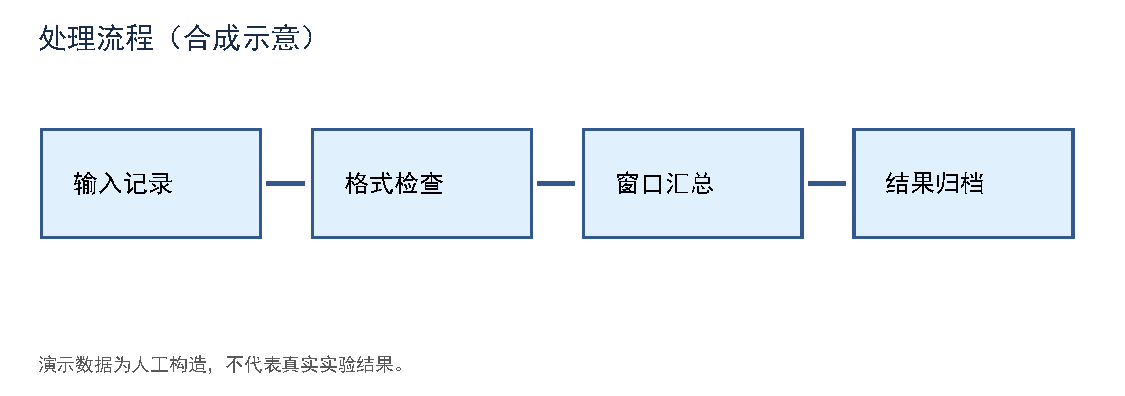
\includegraphics[width=0.95\linewidth]{figs/flow.pdf}
\caption{输入检查与汇总流程。图宽的错误设置不改变图中的流程内容。}
\label{fig:wideflow}
\end{figure}
处理流程先验证各列的类型，再检查同一窗口内的时间顺序。如果检查失败，窗口保持原样并附加状态标记。只有通过检查的窗口进入后续汇总。这样的约定使每个输出都能追溯到输入，也让排版前后的内容核对有明确依据。

展示页面应让标题、说明和图表形成连续的阅读路径。必要的章节分隔、图表内部留白和图注间距应被保留。孤立的大空洞、越过版心的对象以及相互冲突的局部格式则需要单独判断，不能仅凭页面是否填满来评价质量。

\section{状态记录}
比较采用相同的纸张、版心和正文基础字号。两份文档的区别只允许落在已声明的排版命令上。表格数据、图形文件、公式内容和交叉引用在原稿生成后冻结，因此读者可以把注意力放在布局的变化，而不用猜测内容是否也被修改。

\begin{figure}[!b]
\centering
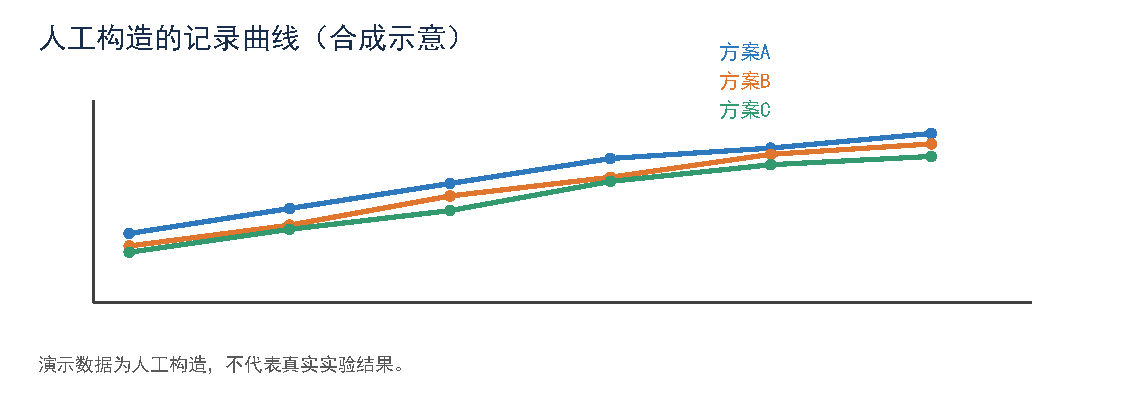
\includegraphics[width=0.95\linewidth]{figs/curves.pdf}
\caption{三组人工构造的示意数值，仅用于保持排版前后的图形内容一致。}
\label{fig:widecurves}
\end{figure}
结果记录分成处理状态和阅读检查两部分。处理状态说明文件能否编译、对象是否完整以及当前仍有哪些日志提示。阅读检查则关注图文距离、标题层次和是否出现遮挡。前者可以重复测量，后者需要结合整页图像检查，不能互相替代。

对于正常范围内的空白，演示不要求进一步压缩。段落之间仍应有适当间隔，插图与图注之间仍应有视觉分离。改变浮动位置时还要重新检查整篇文档，因为前面一个对象的移动可能影响后面多个页面的断点。

\begin{itemize}
\item 窗口边界与输入顺序保持一致。
\item 图文对应关系需要结合整页检查。
\item 图像文件不得在优化时重画或替换。
\end{itemize}
\section{讨论与结论}
本文的目的不是给出真实应用的性能结论，而是形成一个可审计的排版案例。所有操作应记录修改位置、修改理由和验收结果。如果某个候选使全局结果变差，就恢复到修改之前；如果问题无法在既有动作范围内解决，则保留并明确说明。

展示页面应让标题、说明和图表形成连续的阅读路径。必要的章节分隔、图表内部留白和图注间距应被保留。孤立的大空洞、越过版心的对象以及相互冲突的局部格式则需要单独判断，不能仅凭页面是否填满来评价质量。

比较采用相同的纸张、版心和正文基础字号。两份文档的区别只允许落在已声明的排版命令上。表格数据、图形文件、公式内容和交叉引用在原稿生成后冻结，因此读者可以把注意力放在布局的变化，而不用猜测内容是否也被修改。

结果记录分成处理状态和阅读检查两部分。处理状态说明文件能否编译、对象是否完整以及当前仍有哪些日志提示。阅读检查则关注图文距离、标题层次和是否出现遮挡。前者可以重复测量，后者需要结合整页图像检查，不能互相替代。

\end{document}
